\documentclass[base.tex]{subfiles}
\begin{document}
\section{Discussion of results}
We do experiments using different input data in real world and compare the model output with real system output. We calculate the prediction accuracy for each stage and the whole job as well. Results we get are shown below.
\begin{figure}[htbp]
\centering
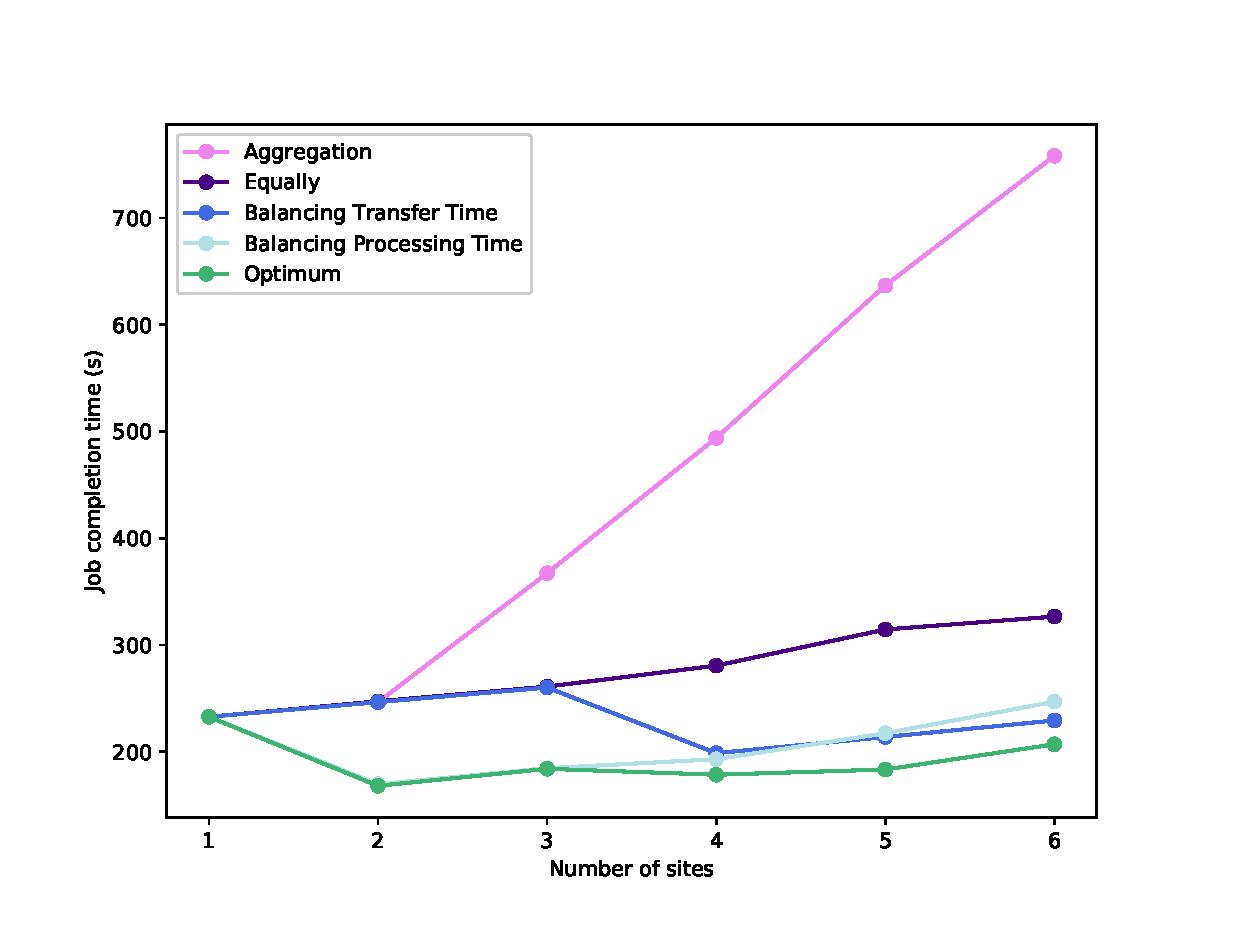
\includegraphics[scale=0.5]{sites_time}
\caption{Job completion time of different strategies varying with number of sites}%\textit{•}}
\label{number of sites}
\end{figure}
As is shown in Figure \ref{number of sites}, we can see that when the number of sites increases, job completion time of every strategies will also increse, especially the Aggregation strategy. The reason for this is that data has increased but the reduce tasks haven't changed. Though the time of stage 1 does not change, the data of reduced task in stage 2 has increased but the parallelism(sites/total data) keeps constant. So we can see that the total time will increase. However completion time of our strategy does not change much when the number of sites changes so when the number of sites increases, our strategy can have less time than others. When there are 6 sites, our strategy reaches 3.68x, 1.58x, 1.11x, 1.19x speedup compared to other 4 strategies. 

\begin{figure}[htbp]
\centering
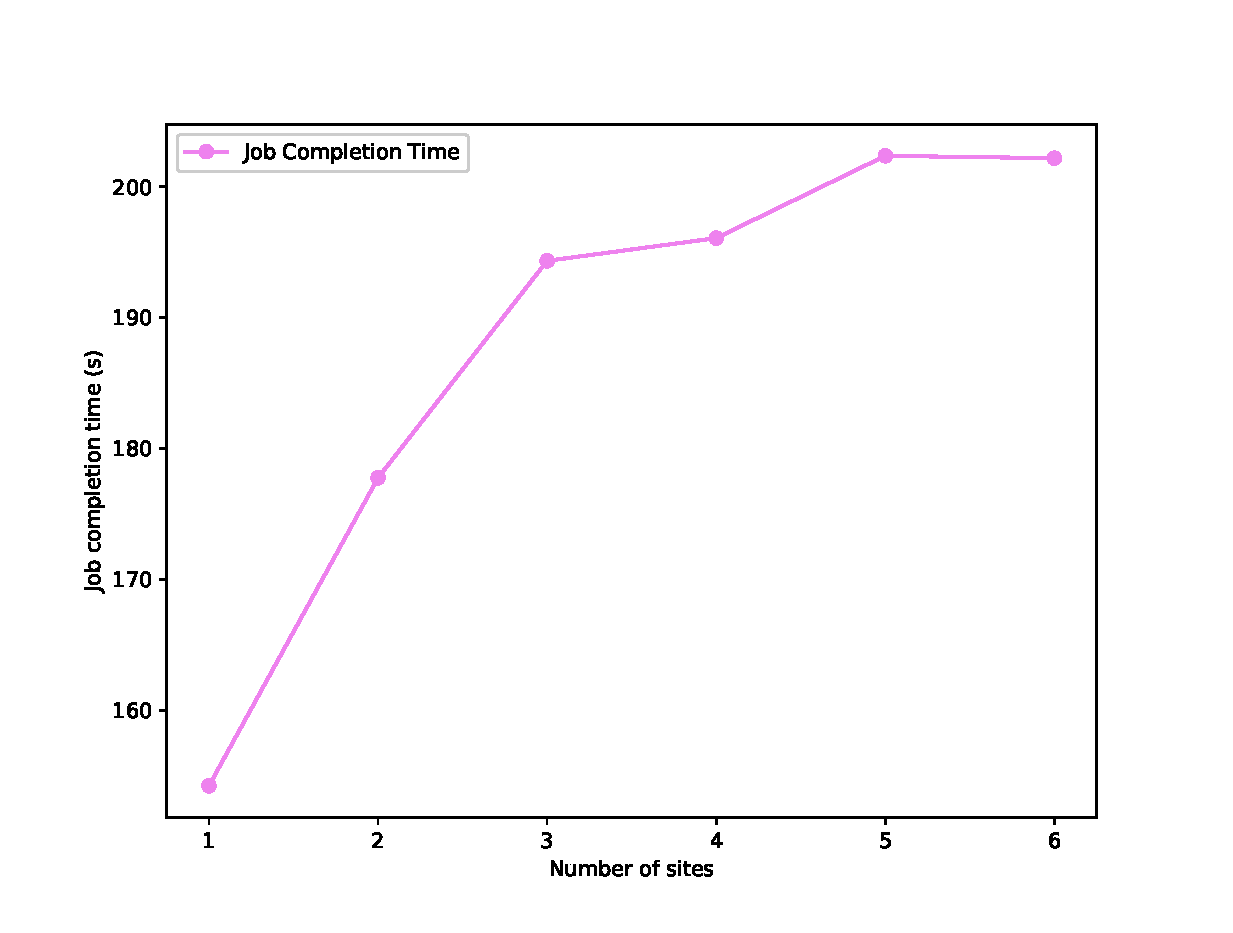
\includegraphics[scale=0.5]{single}
\caption{}%\textit{•}}
\label{single}
\end{figure}

\begin{figure}[htbp]
\centering
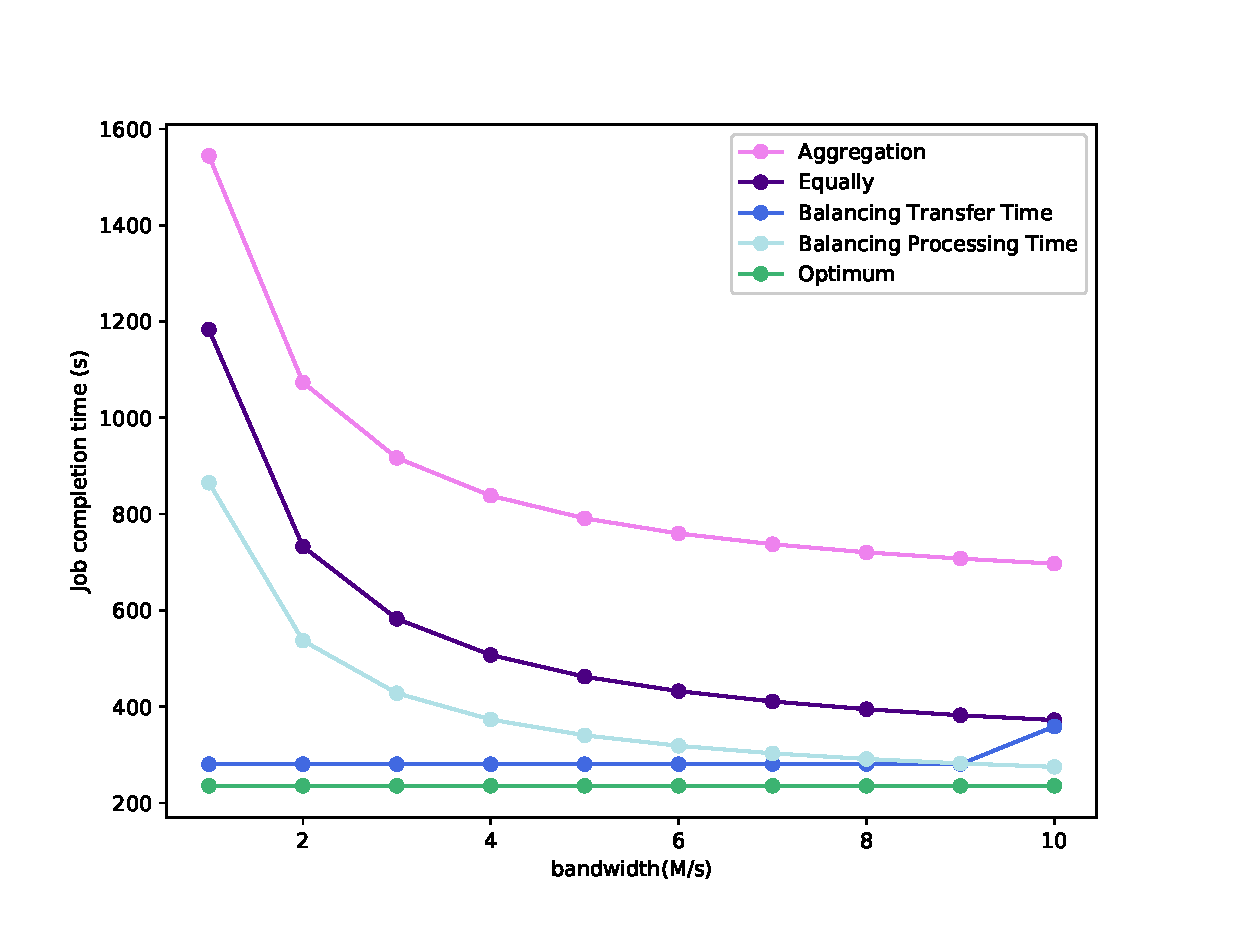
\includegraphics[scale=0.5]{Bandwidth}
\caption{}%\textit{•}}
\label{bandwidth}
\end{figure}

\end{document}
